\documentclass[11pt]{article}
\usepackage[margin=1in]{geometry}
\usepackage{amsmath,amssymb,booktabs,graphicx,hyperref}
\usepackage{xcolor}
\hypersetup{colorlinks=true,linkcolor=blue,urlcolor=blue,citecolor=blue}
\newcommand{\E}{\mathbb E}
\newcommand{\dt}{\Delta t}

\title{Numerical verification of finite-time fluctuation relations\\
for the boundary-driven resonant NLS chain}
\author{}
\date{28 August 2026}

\begin{document}
\maketitle

\section*{Question and scope}

The thermodynamic observable is the total trajectory entropy
\begin{equation}
 \Sigma_{\rm tot}
 =-\frac{Q_L}{T_L}-\frac{Q_R}{T_R}
 +\log\rho(X_0)-\log\rho(X_t),
 \label{eq:total}
\end{equation}
where positive $Q_r$ denotes energy delivered by bath $r$ to the system.
The finite-time integral and detailed fluctuation relations are
\begin{equation}
 \E[e^{-\Sigma_{\rm tot}}]=1,
 \qquad
 \log\frac{p(\Sigma_{\rm tot}=s)}{p(\Sigma_{\rm tot}=-s)}=s.
 \label{eq:ft}
\end{equation}
Two independent experiments now pass their declared numerical gates.  The
accepted conclusion is a numerical verification of finite-time total-entropy
relations for $n=2$.  It is not a mathematical proof and does not establish
the long-chain asymptotic Gallavotti--Cohen symmetry.

\section{Exact discrete forward/reverse path ratio}

The split Cartesian integrator was treated as a discrete Markov process.  For
every boundary Euler bath substep $z\to z'$, the exact Gaussian transition-
kernel ratio was accumulated:
\begin{equation}
 \log\frac{K_T(z,z')}{K_T(\Theta z',\Theta z)}
 =\frac{\lVert-\delta+\gamma F(z')\dt\rVert^2
       -\lVert \delta+\gamma F(z )\dt\rVert^2}
       {4\gamma T\dt},
 \qquad \Theta c=\overline c.
 \label{eq:kernel}
\end{equation}
The implicit-midpoint Hamiltonian map is reversible and volume preserving, so
its path-action contribution cancels.  Forward and conjugate-reverse
trajectories start from the same explicitly normalized product complex-
Gaussian density.  The reverse implementation applies the bath substeps in
reverse order and then advances the already time-reversed state with the same
$+\dt$ Hamiltonian map.

At $(T_L,T_R)=(10,2)$, $n=2$, $t=0.1$, $\dt=10^{-3}$, one million independent
trajectories were generated in each direction.  The results are
\begin{table}[h]
\centering
\begin{tabular}{lrrrr}
\toprule
ensemble & $\log\E e^{-\Sigma}$ & bootstrap 95\% interval
& weight ESS & max. weight fraction \\
\midrule
forward & $-0.003532$ & $[-0.007030,\,0.000244]$
& $226{,}928$ & $6.93\times10^{-4}$ \\
reverse & $-0.002145$ & $[-0.007289,\,0.004550]$
& $87{,}732$ & $2.28\times10^{-3}$ \\
\bottomrule
\end{tabular}
\end{table}

Both IFT intervals include zero.  In 33 symmetric raw-count-qualified bins,
the bidirectional Crooks fit is
\begin{equation}
 \log\frac{p_F(s)}{p_R(-s)}
 =(0.000259\pm0.00151)+(0.993352\pm0.00243)s.
\end{equation}

\begin{figure}[ht]
\centering
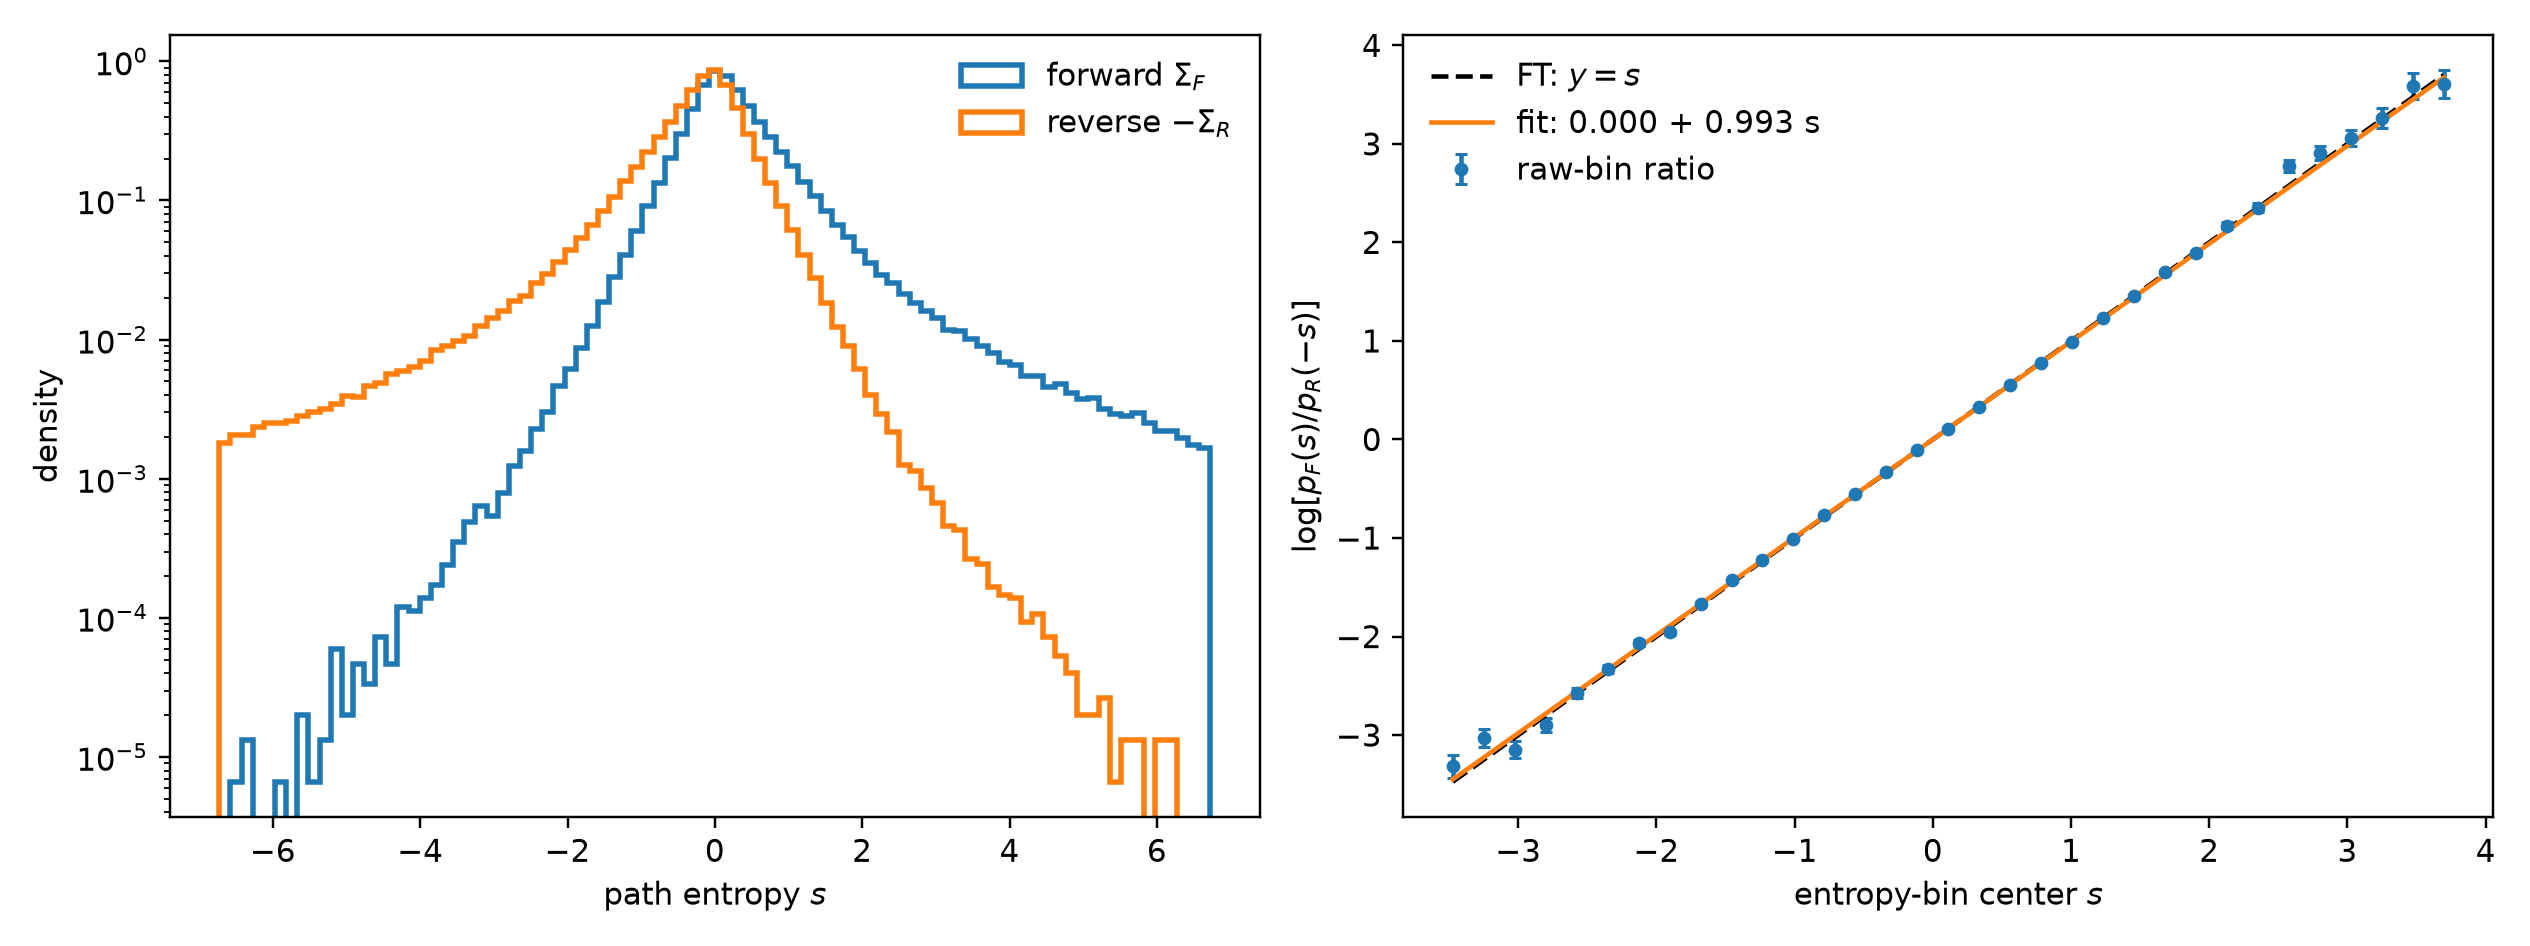
\includegraphics[width=\textwidth]{../../discrete_path_ft_2026-08-28/production_v2/driven_t0p1_dt1e3_N1m_analysis/discrete_path_ft.png}
\caption{Forward/reverse path-entropy distributions and their raw-bin Crooks
ratio.  No pseudocounts enter the fit.}
\label{fig:path-ft}
\end{figure}

The discrete kernel entropy was also compared with the physical heat proxy
$\Sigma_Q=-Q_L/T_L-Q_R/T_R$.  Over
$\dt\in\{2\times10^{-3},10^{-3},5\times10^{-4}\}$, both the absolute mean and
RMS of $\Sigma_K-\Sigma_Q$ converge at first order: the fitted orders are
$0.996$ and $1.004$ forward, and $1.002$ and $0.985$ reverse.  Thus the exact
discrete identity has the expected continuous-time heat interpretation.

\begin{figure}[ht]
\centering
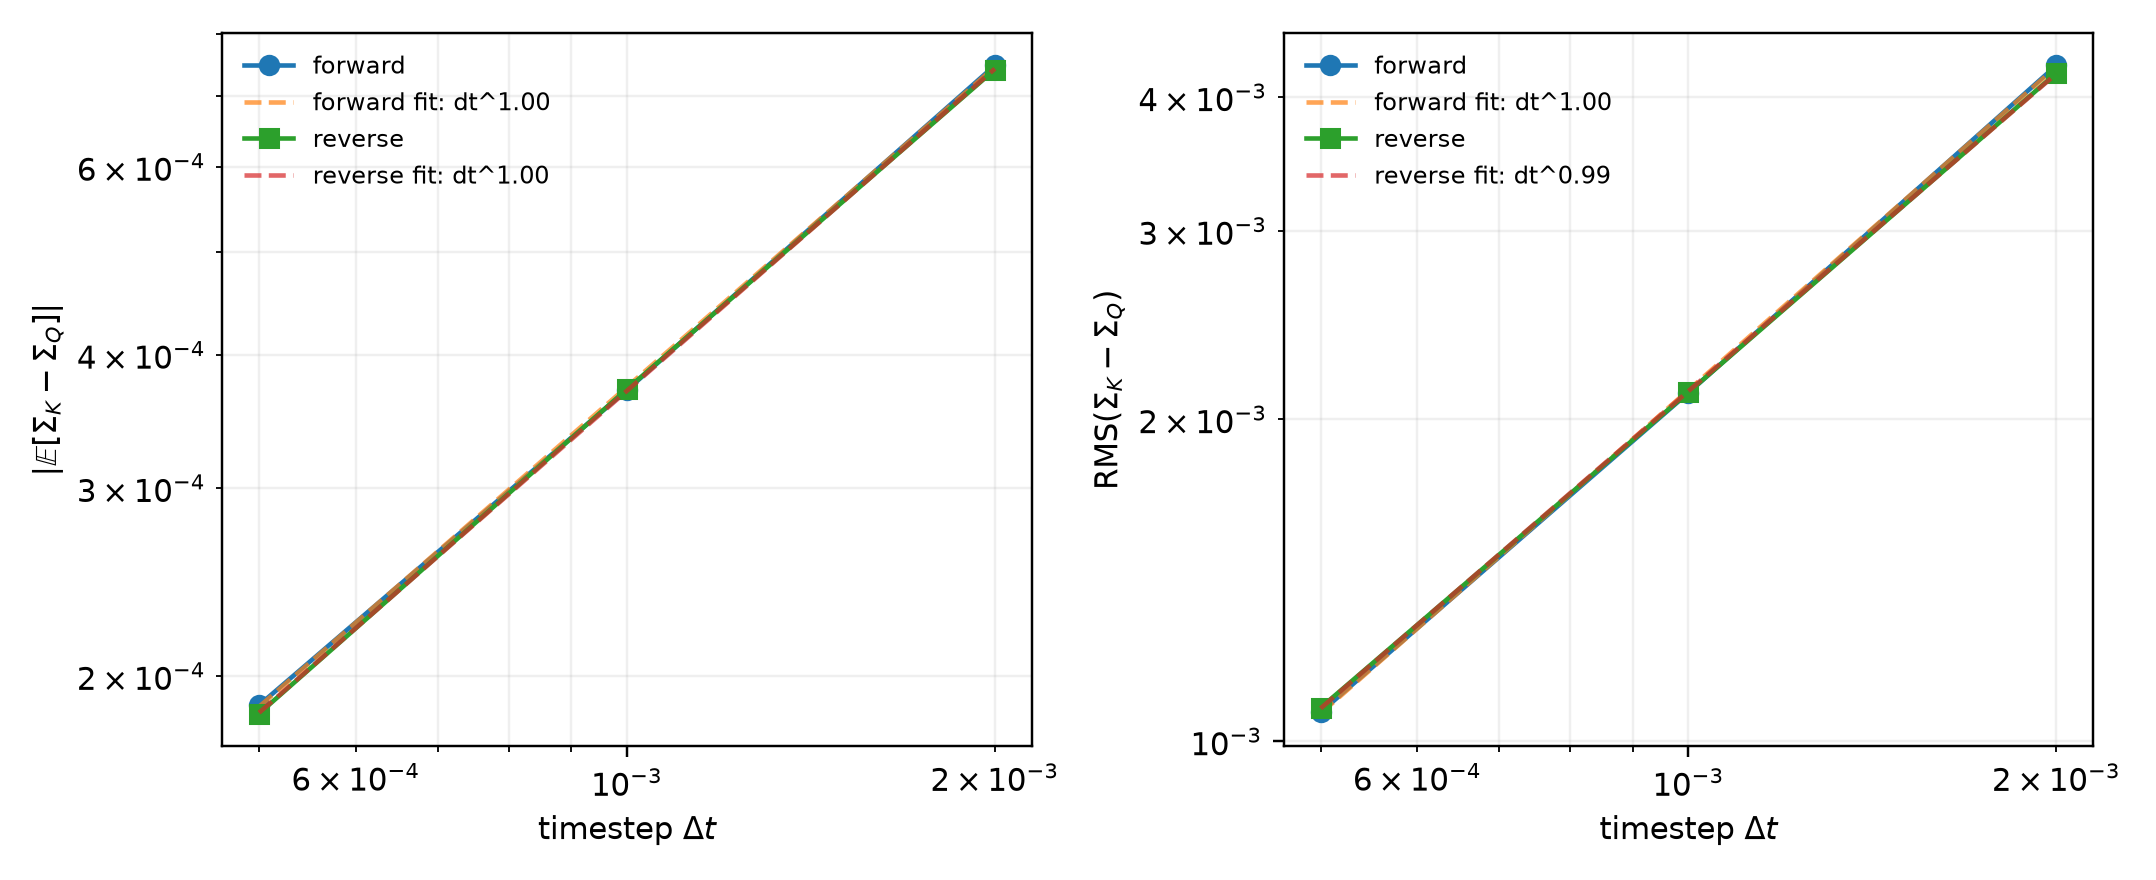
\includegraphics[width=0.9\textwidth]{../../discrete_path_ft_2026-08-28/production_v2/convergence/kernel_heat_timestep_convergence.png}
\caption{First-order convergence of transition-kernel entropy to bath-heat
entropy.}
\label{fig:timestep}
\end{figure}

\clearpage
\section{Driven NESS total entropy at $n=2$}

The second experiment starts from the numerical NESS after burn-in $B=500$.
It contains 64 independent streams and $1{,}048{,}576$ non-overlapping blocks
of length $t=0.1$ at $\dt=5\times10^{-4}$ for both equilibrium $(6,6)$ and
driven $(10,2)$ conditions.  There are no midpoint failures or nonfinite
records.  The RMS absolute first-law residuals are $2.76\times10^{-5}$ and
$3.06\times10^{-5}$, respectively.

For $n=2$, global phase invariance reduces the stationary endpoint density to
the three variables
\[
 u_1=\log|c_1|^2,\qquad u_2=\log|c_2|^2,
 \qquad \theta=2(\arg c_2-\arg c_1).
\]
The density was represented by a normalized action--Fourier exponential
family with action degree two and one angular harmonic.  This family contains
the exact equilibrium form
\[
 \log q(u_1,u_2,\theta)=u_1+u_2-E/T+\mathrm{constant}.
\]
Its structure and regularization were fixed using equilibrium data before it
was applied, cross-fitted by stream, to the driven endpoints.

On an independent equilibrium validation half, the endpoint log-density ratio
has support $0.99979$, RMSE $0.00826$, slope $0.99941$, and correlation
$0.99994$ against the exact Gibbs ratio.  The exact-Gibbs IFT gives
$\log\E e^{-\Sigma}=4.9\times10^{-9}$.

For the driven NESS, the cross-fitted total entropy gives
\begin{equation}
 \log\E e^{-\Sigma_{\rm tot}}=0.002175,
 \qquad 95\%\ \mathrm{CI}=[-0.000744,\,0.005251],
 \qquad \mathrm{ESS}=324{,}604.
\end{equation}
In 60 raw-count-qualified two-sided bins,
\begin{equation}
 \log\frac{p(s)}{p(-s)}
 =-0.02219+(0.99450\pm0.00738)s.
 \label{eq:ness-fit}
\end{equation}
Both tests pass.  The result is stable when the density family is expanded:
\begin{table}[h]
\centering
\begin{tabular}{lrrr}
\toprule
density model & IFT 95\% interval & detailed-FT slope & usable bins \\
\midrule
$D=2,K=1$ & $[-0.000744,\,0.005251]$ & $0.9945\pm0.0074$ & 60 \\
$D=2,K=2$ & $[-0.000206,\,0.005535]$ & $0.9977\pm0.0080$ & 60 \\
$D=3,K=2$ & $[-0.001452,\,0.005606]$ & $1.0035\pm0.0083$ & 61 \\
\bottomrule
\end{tabular}
\end{table}

\begin{figure}[ht]
\centering
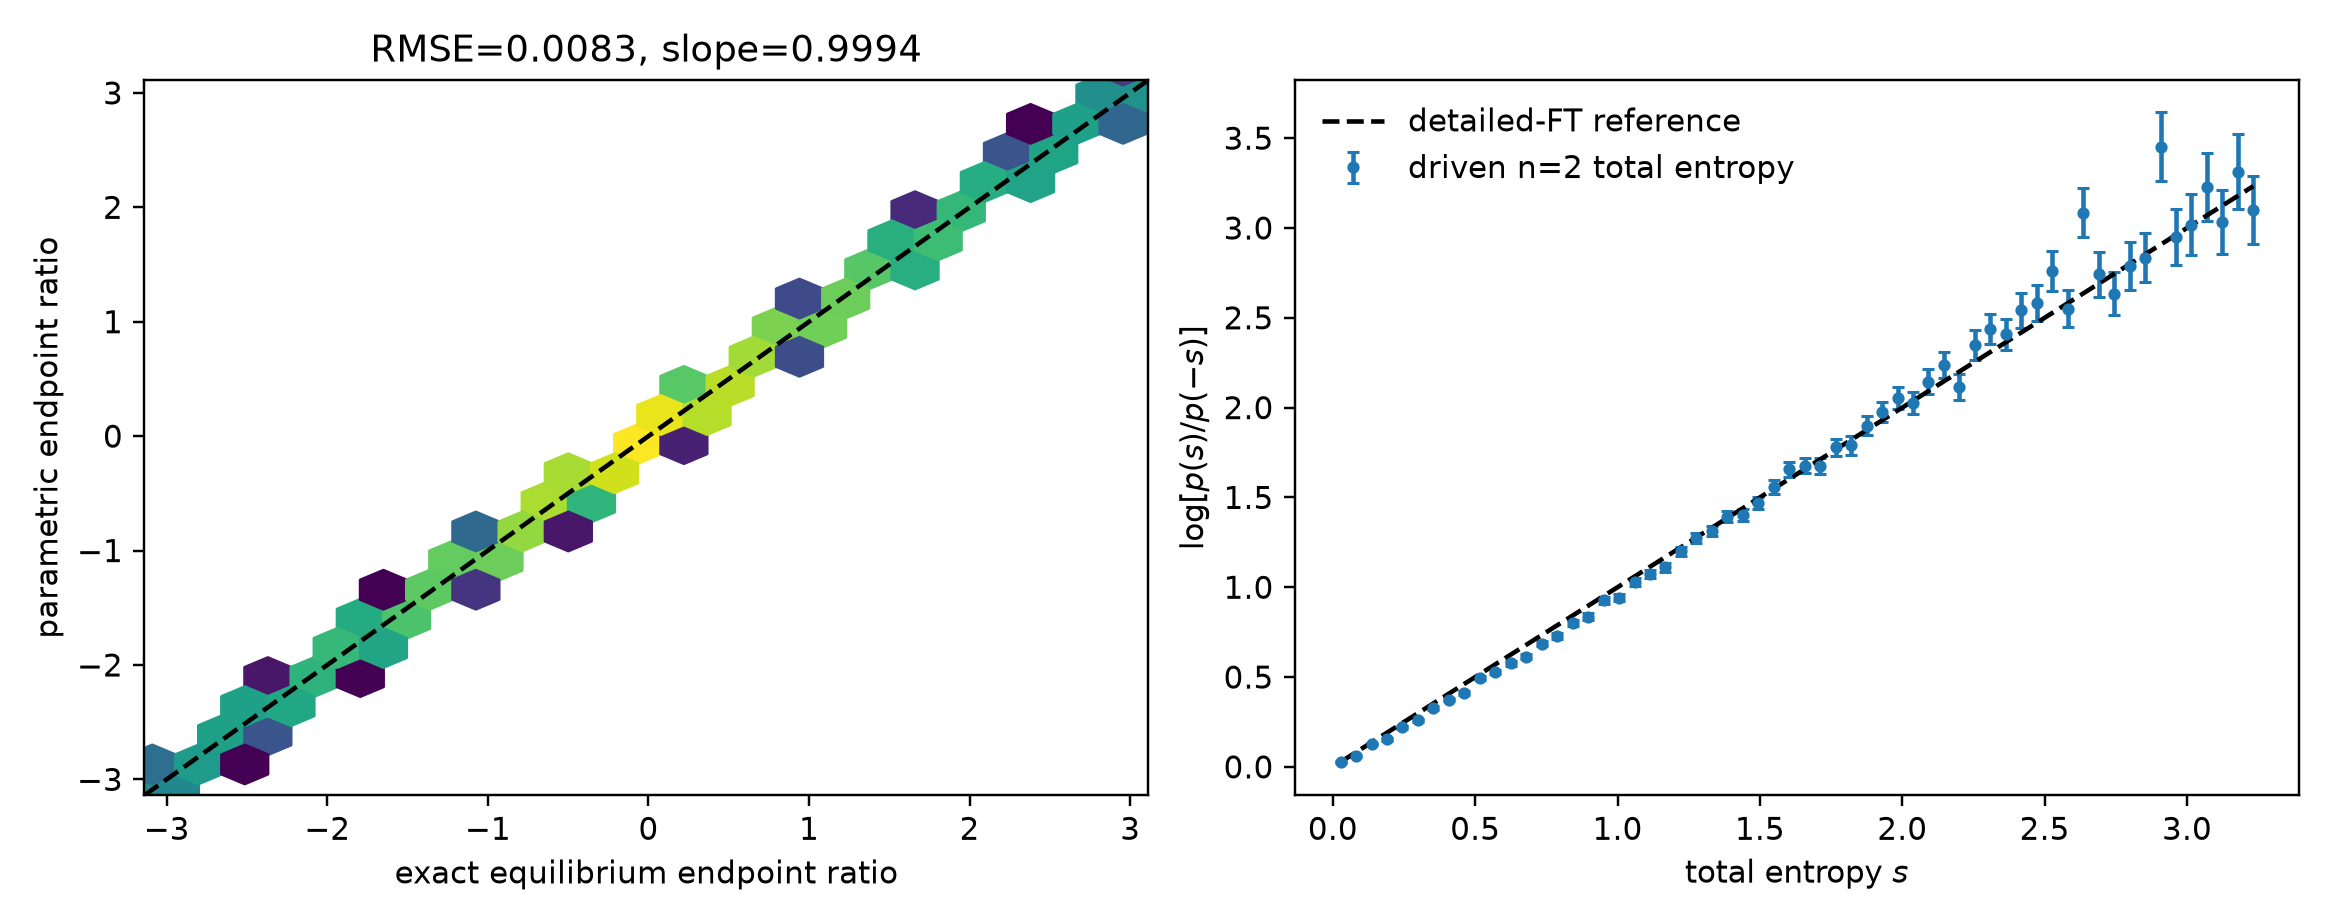
\includegraphics[width=\textwidth]{../../entropy_ft_scgf_2026-08-27/total_entropy_n2_short/parametric_analysis/parametric_total_entropy_ft.png}
\caption{Independent equilibrium endpoint-density validation (left) and the
driven NESS total-entropy detailed fluctuation relation (right).}
\label{fig:ness-ft}
\end{figure}

\section{Interpretation}

The experiments establish the following scoped statement:
\begin{quote}
For the projection-free Cartesian NLS dynamics at $n=2$, the exact discrete
forward/reverse path action satisfies the finite-time integral and detailed
fluctuation relations, and a separate driven-NESS calculation verifies the
same relations for total entropy over $t=0.1$ after independently validating
the stationary endpoint density.
\end{quote}
The older $n=10,20,30,40$ data contain medium entropy only.  Their directly
sampled finite-time symmetry slopes remain below the asymptotic unit reference,
and high-tilt cloning loses genealogical support.  Those results neither
verify nor contradict the long-chain Gallavotti--Cohen relation; they remain a
separate rare-event and endpoint-density problem.

\section*{Reproducibility}

The principal sources are
\texttt{flux/NLS\_discrete\_path\_ft.cpp},
\texttt{flux/analyze\_discrete\_path\_ft.py},
\texttt{flux/analyze\_total\_entropy\_parametric\_n2.py}, and their independent
audit scripts.  Exact commands, fixed gates, summaries, source hashes, and raw
data locations are documented in the corresponding experiment directories.

\begin{thebibliography}{9}
\bibitem{Seifert2005}
U. Seifert, ``Entropy production along a stochastic trajectory and an
integral fluctuation theorem,'' \emph{Phys. Rev. Lett.} 95, 040602 (2005).
\bibitem{LebowitzSpohn1999}
J. L. Lebowitz and H. Spohn, ``A Gallavotti--Cohen-type symmetry in the large
deviation functional for stochastic dynamics,'' \emph{J. Stat. Phys.} 95,
333--365 (1999).
\end{thebibliography}

\end{document}
